%\subsubsection{Desenvolvimento}

	\par Com o ambiente de desenvolvimento pronto, podia-se começar de fato a
desenvolver. Primeiramente foi necessário criar o banco dedados no SGDB. O
banco foi criado, porém sua estrutura não foi definida, pois como será
visto mais adiante o \textit{Hibernate}, possui um mecanismo, que com algumas
configurações, permite a estruturação do banco de dados, de acordo com o
mapeamento objeto relacional. Isto permitirá mudanças na estrutura do banco de
dados e suas tabelas, e até mesmo eventuais correções.

	\par Em seguida foi criado um projeto do tipo \textit{web} no \textit{Eclipse}
com a ajuda do plugin \textit{Maven}. O \textit{archetype} usado foi
\textit{Quick Star WebApp}. Esse Projeto foi criado usando o \textit{Maven}
pois depende de uma quantidade considerável de \textit{frameworks}, e uma das
principais funcionalidades deste plugin, é ajudar na resolução das dependências
de um projeto Java.

	\par Para tal projeto foi necessário a configuração do \texttt{POM.xml} que é o
arquivo utilizado pelo \textit{Maven}. Nele estão contidas as configurações
relativas à compilação do projeto bem como suas dependências.  Na figura
\ref{fig:desws} a seguir pode ser visto o conteúdo do arquivo
\texttt{POM.xml}.

\pagebreak
\begin{figure}[h!]
	\centerline{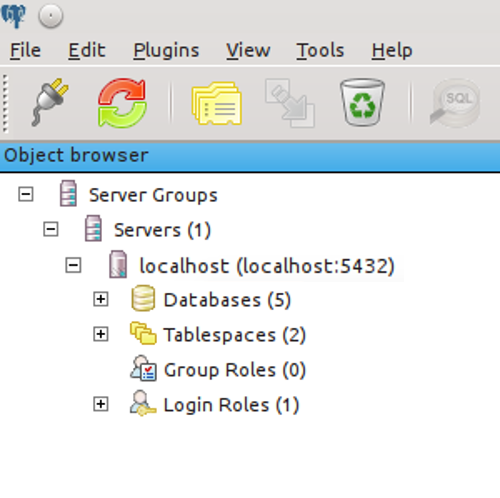
\includegraphics[scale=0.8]{./imagens/2_q_metodologico/4_procedimentos_resultados/43_webservice/432_desenvolvimento/desws.png}}
	\caption[\texttt{pom.xml}]{\texttt{pom.xml}.
		\textbf{Fonte:}Elaborado pelos autores.}
	\label{fig:desws}
\end{figure}

	\par Com a estrutura do projeto devidamente criada foi possível iniciar os
trabalhos com a camada de persistência de dados do projeto. Para tal propósito,
primeiramente foi criado um pacote, onde ficaram contidas as classes que
representam as entidades do ORM. Tal pacote e as classes que a estão
representandos na figura a seguir.
